 
\documentclass[11pt,a4paper]{report}

\usepackage[hidelinks,colorlinks=false]{hyperref}
\usepackage[titletoc,title]{appendix}
\usepackage[nottoc]{tocbibind}
\usepackage{graphicx}
\usepackage{makeidx}
\usepackage{setspace}
\usepackage[margin=1.0in]{geometry}
\usepackage{authblk}
\usepackage{rotating}
\usepackage{cleveref}
\usepackage{float}
\graphicspath{{images/}}

\floatstyle{ruled}
\newfloat{program}{thp}{lop}
\floatname{program}{Program}
 
\begin{document}
	
\title{Final Year Project Report\\ Development and implementation dynamic balance algorithms for bipedal robot locomotion.}
\author{Usvyatsov Mikhail\\Innopolis University\\Kazan\\  ~\\ \normalsize Supervisor: Prof. Eugeni Magid}
\date{\normalsize \today}
\maketitle

\tableofcontents

\newpage

\chapter{Introduction}
Nowadays, humanity invented almost all the devices that are needed for the modern human and society in general. The science is now engaged in the improvement and optimization of existing solutions. These solutions can be traced with trends that are repeated and replicated. For example, the car has 4 wheels while bike - two, and wheels are round, at room there are four walls, etc. This approach is quite good: gain experience, accumulate knowledge and apply them to the latest developments.

According to \cite{pfeifer2007self} it is very important to consider the level of uncertainty of environment where robot works, because its body will interact with this environment. It was common to think before the advent of industrial robots that robots should look like humans. The first use of the word "robot" referred to the humanoid machines that were supposed to serve a human. However, from the very beginning almost every automatic device intended for production and other operations normally performed by the human was called robot. Intensive development of robots begun after the Second World War, which was associated with the emergence of the nuclear industry.

Robots in today's presentation (autonomous device that performs some work in automatic mode) can be attributed with machine "Lunokhod-1", created in 1966. This is the first in the history machine that worked on the surface of Moon (1970). Recent tendency in robotics is replacing people not only in manufacturing but also in the military sphere. Constantly emerging information about the achievements of the leading countries in the development of military land, underwater robots and unmanned aerial vehicles is evidenced for this thesis. The era of development of  bipedal humanoid walking robots develops nowadays.

The trend towards automation is a core part of progress. Automation reduces the cost of technical processes and the risk to humans. Therefore, the research and implementation of patterns in this task are on the cutting edge of science and technology and require special attention and investment in its development. Every year in the world there are more and more situations requiring people perform a wide variety of work in heavy, dangerous, and sometimes incompatible with the life conditions. In response, there are new tools of extreme robotics. However, for the most part they are very similar to each other. Usually, to perform the task on the ground is a autonomous wheeled or tracked vehicle with installed manipulator. Control is carried out remotely by radio or cable. These robots are produced for more than a dozen years. Engineers during that time accumulated a lot of experience in their development and applications, in some cases, very effective. However, it is undeniable that this technique has (like any other) limited scope of application. And as before, the people at the risk of life and limb, work in the rubbles, on fire, in terms of chemical, biological and radioactive contamination, are fighting against criminals and terrorists. Moreover, most of all this actions are situated not in the area of open field but in the buildings and various facilities, cabins and rooms of various equipment,  generally in conditions originally created for humans, given its two arms and two legs, the typical size, weight, and, if I may say so, the kinematics of the body. For this reason other areas of extreme robotics are developing now. One of this is a robotic system including a anthropomorphic bipedal walking robot. Kinematics, size and weight  similar to human characteristics, is equipped with an energy source, communication channel with the control station, and powerful autonomous control system, allowing to perform some action in the supervisory or automatic mode (independent transportation from the place of work in the absence of communication). Such a robot can have significant advantages in a workspace adapted for humans.

\chapter{Literature review}
Bipedal locomotion is a very complex task and according to \cite{erbatur2002study} it is described by nontrivial dynamics. It still doesn't have complete general solution however the research of this has a long history. The development of the models starts from the inverted pendulum model of human walking and goes to the complex approach of actuated passive walking with ZMP control.\\
According to \cite{wright2014intelligent}, there are 5 groups of approaches to the problem of locomotion control. There are:
\begin{enumerate}
	\item Analytical
	\item Central Pattern Generator (CPG)
	\item Neural Networks
	\item Hidden Markov Model (HMM)
	\item Rule based
\end{enumerate}

\section{Analytical approach}
The oldest one and also the most studied group is analytical one. It requires the knowledge of general form that locomotion should take.

For bipedal locomotion it requires the following steps:
\begin{enumerate}
	\item Apply stability constraints
	\item Design gait algorithm (including double support, single support and no-support phases \cite{wright2014intelligent}).
	\item Solve remaining degrees of freedom (DoF) with Inverse Kinematics (IK).
\end{enumerate}

According to \cite{tang2008analysis}, the most natural method that represents the human body is inverted pendulum.
Inverted pendulum model of human balance problem is one of the most primitive and old example of analytical approach \cite{winter1995human}. It stated that control of the balance can be achieved with two components: ankle mechanism (invertors/evertors) and hip load/unloading mechanism. In different positions each of the mechanism plays a different role. Thus in tandem or intermediate position balance is achieved by invertors/evertors mechanism while direction is controlled by hip load/unloading mechanism. It doubts on commonly used condition: reaction force of the floor has to go thought center of gravity of the robot. It was stated, that modern bio-mechanical studies show that there are angular moments around center of gravity. 
Thus this approach is too approximate and it is not very accurate.
Moreover, according to \cite{kuo2007six} six determinants theory\cite{inman1953major} well described by inverted pendulum model needs more energy to control the mechanism and this problem can be solved by passive dynamic walking machines, that need external energy only for transition from one pendular stance leg to another. In \cite{collins2005bipedal} such architecture was considered. There robot was able to move forward at constant not very high speed and author mentioned that the gait of the robot was human like. Human gait is desirable because of its energy effectiveness \cite{golliday1977approach}.\\
Furthermore, \cite{anderson2005powered} summaries principles that allows to combine passive dynamic control with powered bipeds. The results show that the gait become energy efficient however it implies further work on robustness and flexibility of walking\\

In 1970 Miomir Vukobratovic proposed Zero Moment Point (ZMP), a theoretical model to explain biped locomotion. Also ZMP is a basic dynamical stability constraint.
According to \cite{manchester2011stable} we can divide all the existing humanoid bipedal walking robots into two big groups: ZMP-controlled ones and passive - dynamic walkers.\\
Zero moment point is a concept related with dynamics and control of legged locomotion for humanoid robots. It specifies the point with respect to which dynamic reaction force at the contact of the foot with the ground does not produce any moment in the horizontal direction, i.e. the point where the total of horizontal inertia and gravity forces equals to zero.
Miomir Vukobratovic in \cite{vukobratovic2004zero} defines ZMP (Zero Moment Point) as a point in which we can reduce all the forces and moments with one single force $F_a$ and moment $M_a$ respectively  \cref{fig:1}.
	
	\begin{figure}[h!]
		\vspace{-0.2cm}
		\centering
		{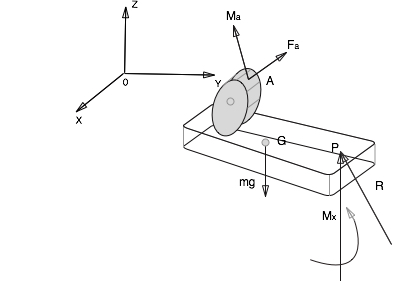
\includegraphics[width=0.7\textwidth]{1}}
		\caption{The sole with acting forces on it}
		\label{fig:1}
		\vspace{-0.1cm}
	\end{figure}

On the figure above we consider only the sole separately from other parts of the leg. It has its own center of gravity G. At point P there is resulting ground reaction that maintains the construction in the equilibrium. The force of ground reaction R and moment M consists of its three components ($R_x$, $R_y$, $R_z$) and ($M_x$, $M_y$, $M_z$) respectively. Horizontal components of R should compensate friction force in the point of contact. Thus, the horizontal reaction of force ($R_x$, $R_y$) represents 
friction force that compensate horizontal component of $F_a$. In the same time the moment $M_z$ represents friction reaction forces \cref{fig:2} that compensates vertical component of $M_a$ and the moment induced by $F_a$. \cite{vukobratovic2004zero}

	\begin{figure}[h!]
		\vspace{-0.2cm}
		\centering
		{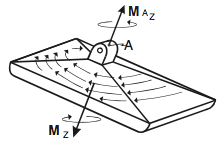
\includegraphics[width=0.7\textwidth]{2}}
		\caption{Rotational moment in the sole}
		\label{fig:2}
		\vspace{-0.1cm}
	\end{figure}

According to \cite{kajita2003biped}, this ZMP should be on the foot. The problem is that we cannot manipulate the foot directly \cite{mitobe2000control}. According to \cite{vukobratovic2004zero} we can do it by ensuring the appropriate dynamics of the mechanism above the foot. If the resulting force in ZMP lies not in vertical direction (conditions from the paragraph above doesn't hold and R and $M_z$ doesn't compensate correspondent components of $F_a$ and $M_a$) than foot will slide. It means that dynamical stability was not achieved due to the fact, that there is a rotational moment that will affect the robot. On the other hand, in \cite{sardain2004forces} it was proven: if ZMP was achieved in the polygon of foot and moreover it coincides with the contact point, than robot is stable, due to the fact, that all the resulting forces lies in vertical direction. During the walk the position of ZMP should be computed simultaneously and the main problem of control is to keep ZMP and contact point to be coincided inside the support polygon of contact foot with the ground.
The name zero moment point relates to the fact, that dynamical stability is maintained if horizontal components $M_x$ and $M_y$ are both equal to zero.
	
	\begin{equation}
		M_x = M_y = 0
	\end{equation}

In the point P there should exist such equivalent force R and vertical moment $M_z$ that compensate the force reaction of the ground and maintains the stability of the construction. If we want to achieve the dynamical stability, that the following equations holds:

	\begin{equation}
		R + F_a + mg = 0
	\end{equation}

Where $m$ is a foot mass. In \cite{vukobratovic2004zero} there is defined  point O - the origin coordinates frame from which we can define radius vectors $\vec{OP}$, $\vec{OG}$ and $\vec{OA}$ where A is a point of ankle joint.

	\begin{equation}
		\vec{OP} \times \vec{R} + \vec{OG} \times mg + M_A + M_z + \vec{OA} \times F_a = 0
	\end{equation}

Placing the origin frame into the point P and making a projection on the horizontal plane gives us the following equations: 

	\begin{equation}
		(\vec{OP} \times \vec{R})^H + \vec{OG} \times mg + M_A^H + (\vec{OA} \times F_a)^H = 0
	\end{equation}

According to \cite{vukobratovic2004zero} equation (4) represents the foot equilibrium. However ot doesn't solve the problem, that it is still unknown whether for the given motion of mechanism it is in the equilibrium. It is only of ZMP lies inside the support polygon.

In \cite{dekker2009zero} it was stated, that we have to make the following assumptions in order to compute the position of ZMP:

	\begin{enumerate}
		\item
			The bipedal robot consists of n rigid links.
		\item
			All kinematic information, such as position of CoM, link orientation, velocities, etc. are known and calculated by forward kinematics.
		\item
			The floor is rigid and motionless.
		\item
			The feet cannot slide over the floor surface.
		\item
			All joints are actively actuated.
	\end{enumerate}
	
With this constraints we can define the mass of the robot as:
	
	\begin{equation}
		m_{robot} = \sum^n_{i=1}{m_i}
	\end{equation}

In \cite{dekker2009zero} it was considered schematic bipedal robot to derive the coordinates of ZMP [Fig. 3]

	\begin{figure}[h!]
		\vspace{-0.2cm}
		\centering
		{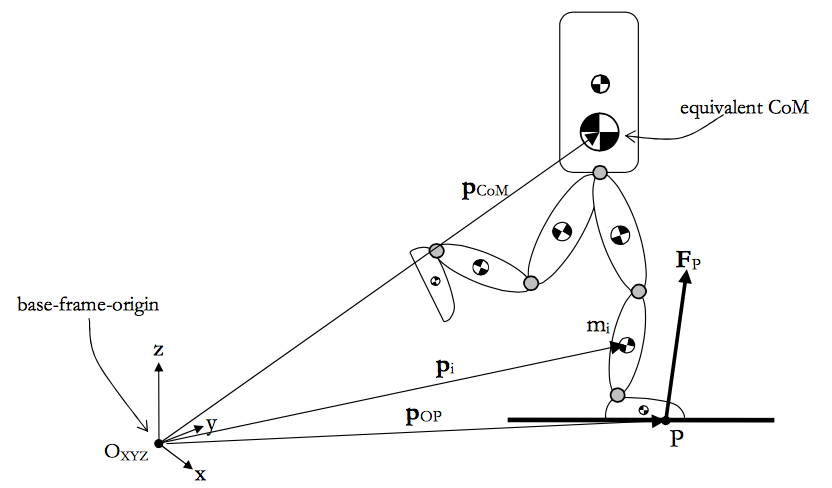
\includegraphics[width=0.7\textwidth]{3}}
		\caption{Rotational moment in the sole \cite{dekker2009zero}}
		\label{fig:3}
		\vspace{-0.1cm}
	\end{figure}

Here $p_i$ are the distances between base frame and equivalent center of mass of i-link. From this total linear momentum P is:
	
	\begin{equation}
		P = \sum^n_{i=1}{m_i \dot{p_i}}
	\end{equation}
And total angular momentum H is:
	\begin{equation}
		H = \sum^n_{i=1}{\dot{p_i} \times m_i \dot{p_i} + I_i \omega_i}
	\end{equation}

Where $\omega_i$ is a angular velocity and $I_i$ is inertia tensor that is computed as:
	\begin{equation}
		I_i = R_i I_i R_i^T
	\end{equation}
Here $R_i$ is a rotation matrix from i-link w.r.t. the origin base frame and $I_i$ is a inertia matrix of i-link w.r.t. the link frame origin attached to their links.

Taking the derivative from 6 and 7 we have got:
	\begin{equation}
		\dot{P} = \sum^n_{i=1}{m_i \ddot{p_i}}
	\end{equation}
	\begin{equation}
		\dot{H} = \sum^n_{i=1}{\ddot{p_i} \times m_i \dot{p_i} + \dot{p_i} \times m_i \ddot{p_i} + I_i \dot{\omega_i}} + \omega_i \times I_i \omega_i
	\end{equation}

In \cite{manchester2011stable} it was mentioned that ZMP approach give us the solution that is based on the principle of dynamical stability, however it is not energy efficient. It requires simultaneous control over all the joints of the robot. The method that was described in \cite{collins2001three} is called passive-walker dynamics and it uses gravity forces to reduce the amount of necessary energy to control the robot.\\
It was mentioned earlier that active control of the robot should be performed with applying dynamical stability principle, elsewhere the robot will loose the balance and fall. So, it makes sense to apply passive-walker dynamics with ZMP based control. According to \cite{vukobratovic2004zero} ZMP method is the most well known and so it is necessary to start with it. \\
According to \cite{vukobratovic2004zero} the most important task in the bipedal locomotion is to maintain dynamical stability. It can be accomplished if the foot have a full contact with the ground, it means, that the contact is not only in the edge or in the point. Moreover it shows that ZMP position depends on the robot dynamics: the resulting force in the contact polygon and total moment there. So, during the motion the position of ZMP changes and there are situations when ZMP reaches the edge of support polygon. In these situations if additional moments appear, robot will rotate around foot edge and collapse. \cite{vukobratovic2004zero} suggests the way to measure the load on the sole via force sensors on it. The algorithm of ZMP control is quite obvious. Compute wanted ZMP coordinates, measure the error and apply correcting signal. Very important notion is about Center of Pressure (CoP). According to \cite{vukobratovic2004zero} the pressure between foot and the ground can be replaced with the force applied in CoP. With this we can define stability condition as ZMP and CoP coincident. Usually ZMP is required to be under the center of the foot during the single support phase, transitioning to the other foot in the double support phase.\\
ASIMO - bipedal robot of Honda company was build on top of this theory and the history of its evolution is described in \cite{hirai1998development}. Nowadays ASIMO is one of the most developed robot, it can interact with human and perform different task starting with playing footboll and finishing stair climbing.\\ 
In \cite{kim2012zmp} it was mentioned the new approach to solve ZMP control problem. Using neural network trained with back propagation method was used to control the position of the robot given the errors between ZMP position and CoP.
In \cite{goswami1999postural} the problem of foot rotation was formulated. The author introduced the Foot-Rotation Indicator (FRI) the point, that can leave the support polygon and describe the impeding rotation. When FRI lies outside the support polygon it means that there is rotational moment and acting on the foot that helps control instability of the gait.

\section{Central Pattern Generator}

Experiment in \cite{grillner1975locomotion} shown that reflexes are significant for locomotion. During reverse engineering it was found neural network that controls locomotion. It was found in spinal regions and it was the reason to name this approach as Central Pattern Generator.\\
This approach for gait generation was considered in \cite{miyakoshi1998three}. There neural oscillator was used for generation biped motions. Human like gait was achieved by robot with small Degree of Freedom (DoF). The idea of this oscillator was to build robust system that perform simple control with minimum structure of neural architecture that can be interesting for high DoF robot.\\
A detailed examination of a biological CPG from an engineering perspective was conducted in \cite{zhu2006central} but, for most applications, the neuron pair is approximated with a pair of differential equations \cite{wright2014intelligent}.

Also \cite{wright2014intelligent} considers two types of oscillators:

\begin{enumerate}
	\item Simple Sinusoidal Oscillator\\
	That is too simple for bipedal locomotion because it is impossible to maintain dynamical stability criteria with this type of oscillations.
	\item Systems of Differential Equations\\
	Analysis of biological CPGs has identified oscillators made from pairs of mutually inhibiting neurons \cite{grillner1995neural}. These oscillators are able to generate different gaits and produces various solutions from sinusoidal to more complex forms. It can control biped even on the rough ground. Matsuoka, Van der Pol, Amari-Hopfield, Hopf, Ellias shunting oscillators were used in numerous works and in \cite{lee2007construction} Generalized CPGs was introduced. 
\end{enumerate} 

\section{Neural Networks}
Despite of the fact that oscillators can be described as a neural network they do not require any input for their work. Canonical Neural Networks (NN) have input data and output. There are several groups of NN.

\subsection{Feed-Forward Networks}
In this networks each neuron has its own connection and transfer function. They a ready for state motion generation.  Input data is current kinematics and sensory data. They can generate not state based trajectories only with time input. Multi-layer perceptron (MLP) is one of such models. They have from three (input, output, hidden) layers and can have more hidden ones. According to \cite{vundavilli2010dynamically}, two MLPs were used to specify parameters of a bipedal ditch crossing gait trained with Genetic Algorithm (GA) produced the best solution in terms of stability. It was more stable and efficient than one from a fully analytical approach, and slightly better than the result obtained with a fuzzy logic based method. Activation function is sigmoid.\\
Radial Basis Function Network is another example of Feed-Forward Networks (FFN). Activation function is usually Gaussian or Euclidean. Neurons in hidden layers connected only with small part of input neurons. For this reason two types of vectors are necessary: wights vector and centre vector which is the same dimension as input. Each vector responds if it is close to its weight vector. Output neurones are the functions of linear combinations of outputs of network and their wighted connections.
It was used for hexapod locomotion \cite{ilg1995learning}.\\
A Cerebellar Model Articulation Controller (CMAC) is a type of associative memory network based on cerebellum \cite{albus1975new}. Input space is continuous and divided into hyper-rectangles. So input should be located at one rectangle in the moment. Numerous hidden layers are slightly moved rectangles. Hence rectangles will overlap on different layers. The output for each layer is wighted sum of activated rectangles. The CMACs successfully learned the movement patterns and showed resilience to perturbation (including on uneven or slippery floors), thereby translating a rigid analytical solution into an adaptable one \cite{sabourin2005robustness}.
\subsection{Recurrent Networks}
The structure of such networks is more complicated that FFN. Thus we can produce more complex patterns and handle different type input. 
\section{Hidden Markov Model}
\section{Rule based approach}
\newpage
\chapter{Theoretical Foundations: Background Material}
\newpage
\chapter{Formal Model: Theoretical Development}
\newpage
\chapter{Algorithmic Considerations}
\newpage
\chapter{Implementation Issues}
\newpage
\chapter{Evaluation}
\newpage
\chapter{Future Work}
\newpage
\chapter{Description of the Project Workplan}
\begin{enumerate}
	\item
	Literature review.
	\item
	Compare different approaches to bipedal locomotion.
	
	Bipedal locomotion consists of several phases. There are walking and staying parts. Each of this part requires different type of stability. If robot is statically stable, then it wouldn't require any energy while it stays. On the other hand, during walking bipedal robot should be stable, but previous characteristic doesn't provide this property. So we came up with the idea of dynamical stability, that will allow the robot to move. 
	There are several ways to achieve it. E.g. neural networks, ZMP, passive walking, capture point, to name a only few.
	\item
	Choose the most appropriate approach.
	
	The process of bipedal walking consists of continuous falling of the robot but it have to prevent it on time and change the phase. From this point of view it doesn't seems that neural networks are the good idea because we can describe the model precisely. More over bipedal robot is interesting because of its anthropomorphism because of it robot can be placed in the same environment as a human. This requirements make us think about the approach that is energy and computationally efficient and also provide a good precision of walking in several degrees of uncertainty.  
	\item
	Make the computer model of the robot.
	
	During the development we should compare several models ща the control, also mistakes are inevitable. Thus virtual simulation environment is necessary to prevent robot failure and reduce the time of problems identifying.
	\item
	Implement algorithm on this model.
	
	Algorithm should be implemented in simulator to prove that it allows control the entire model.  
\end{enumerate}

\bibliographystyle{unsrt}
\bibliography{robotics}
  
\end{document}

